% todo: add citations
\section{Architecture encodeur--décodeur}

Les lacunes des \glspl{mlp} sont en large partie le résultat du traitement séparé des parties des séquences.
Dans la production de l'élément (ou bloc) courant de la sortie,
un \gls{mlp} se base uniquement sur l'élément (ou bloc) correspondant de l'entrée.
L'équation~\ref{eq.mlp-seq-prod} l'illustre pour une entrée \(x = (x_1, x_2, \cdots, x_n)\)
et une sortie \(y = (y_1, y_2, \cdots, y_m)\).
%%
\begin{equation}
    \label{eq.mlp-seq-prod}
    y_j = f(x_i, x_{i+1}, \cdots, x_{i+\ell}) \qquad 1 \le j \le m
\end{equation}
%%
En plus de l'hypothèse implicite de l'existence d'une telle correspondance,
cela suppose que les éléments d'une séquence sont complètement indépendants les uns des autres.
Cette dernière hypothèse n'est presque jamais vérifiée. 

Une façon naturelle de combler ces lacunes est d'abandonner le traitement par bloc de l'entrée.
Tout élément de la séquence de sortie est considéré comme fonction de la séquence d'entrée toute entière.
L'équation~\ref{eq.yj-of-x} montre cette approche sur l'exemple précédent~\cite{Stahlberg_2020}.
%%
\begin{equation}
    \label{eq.yj-of-x}
    y_j = f(x) = f(x_1, x_2, \cdots, x_n) \qquad 1 \le j \le m
\end{equation}
%%
L'architecture encodeur--décodeur y parvient en combinant deux modules : un encodeur et un décodeur.
L'encodeur consomme la suite donnée en entrée et produit un vecteur de dimension fixe qui la représente%
~\footnote{Ce vecteur est appelé un vecteur de contexte, vecteur de pensée ou encore un encodage.}.
Le décodeur consomme ce vecteur et produit la sortie (voir Figure~\ref{fig.encoder-decoder}).
%%
\begin{figure}[hbt]
    \centering
    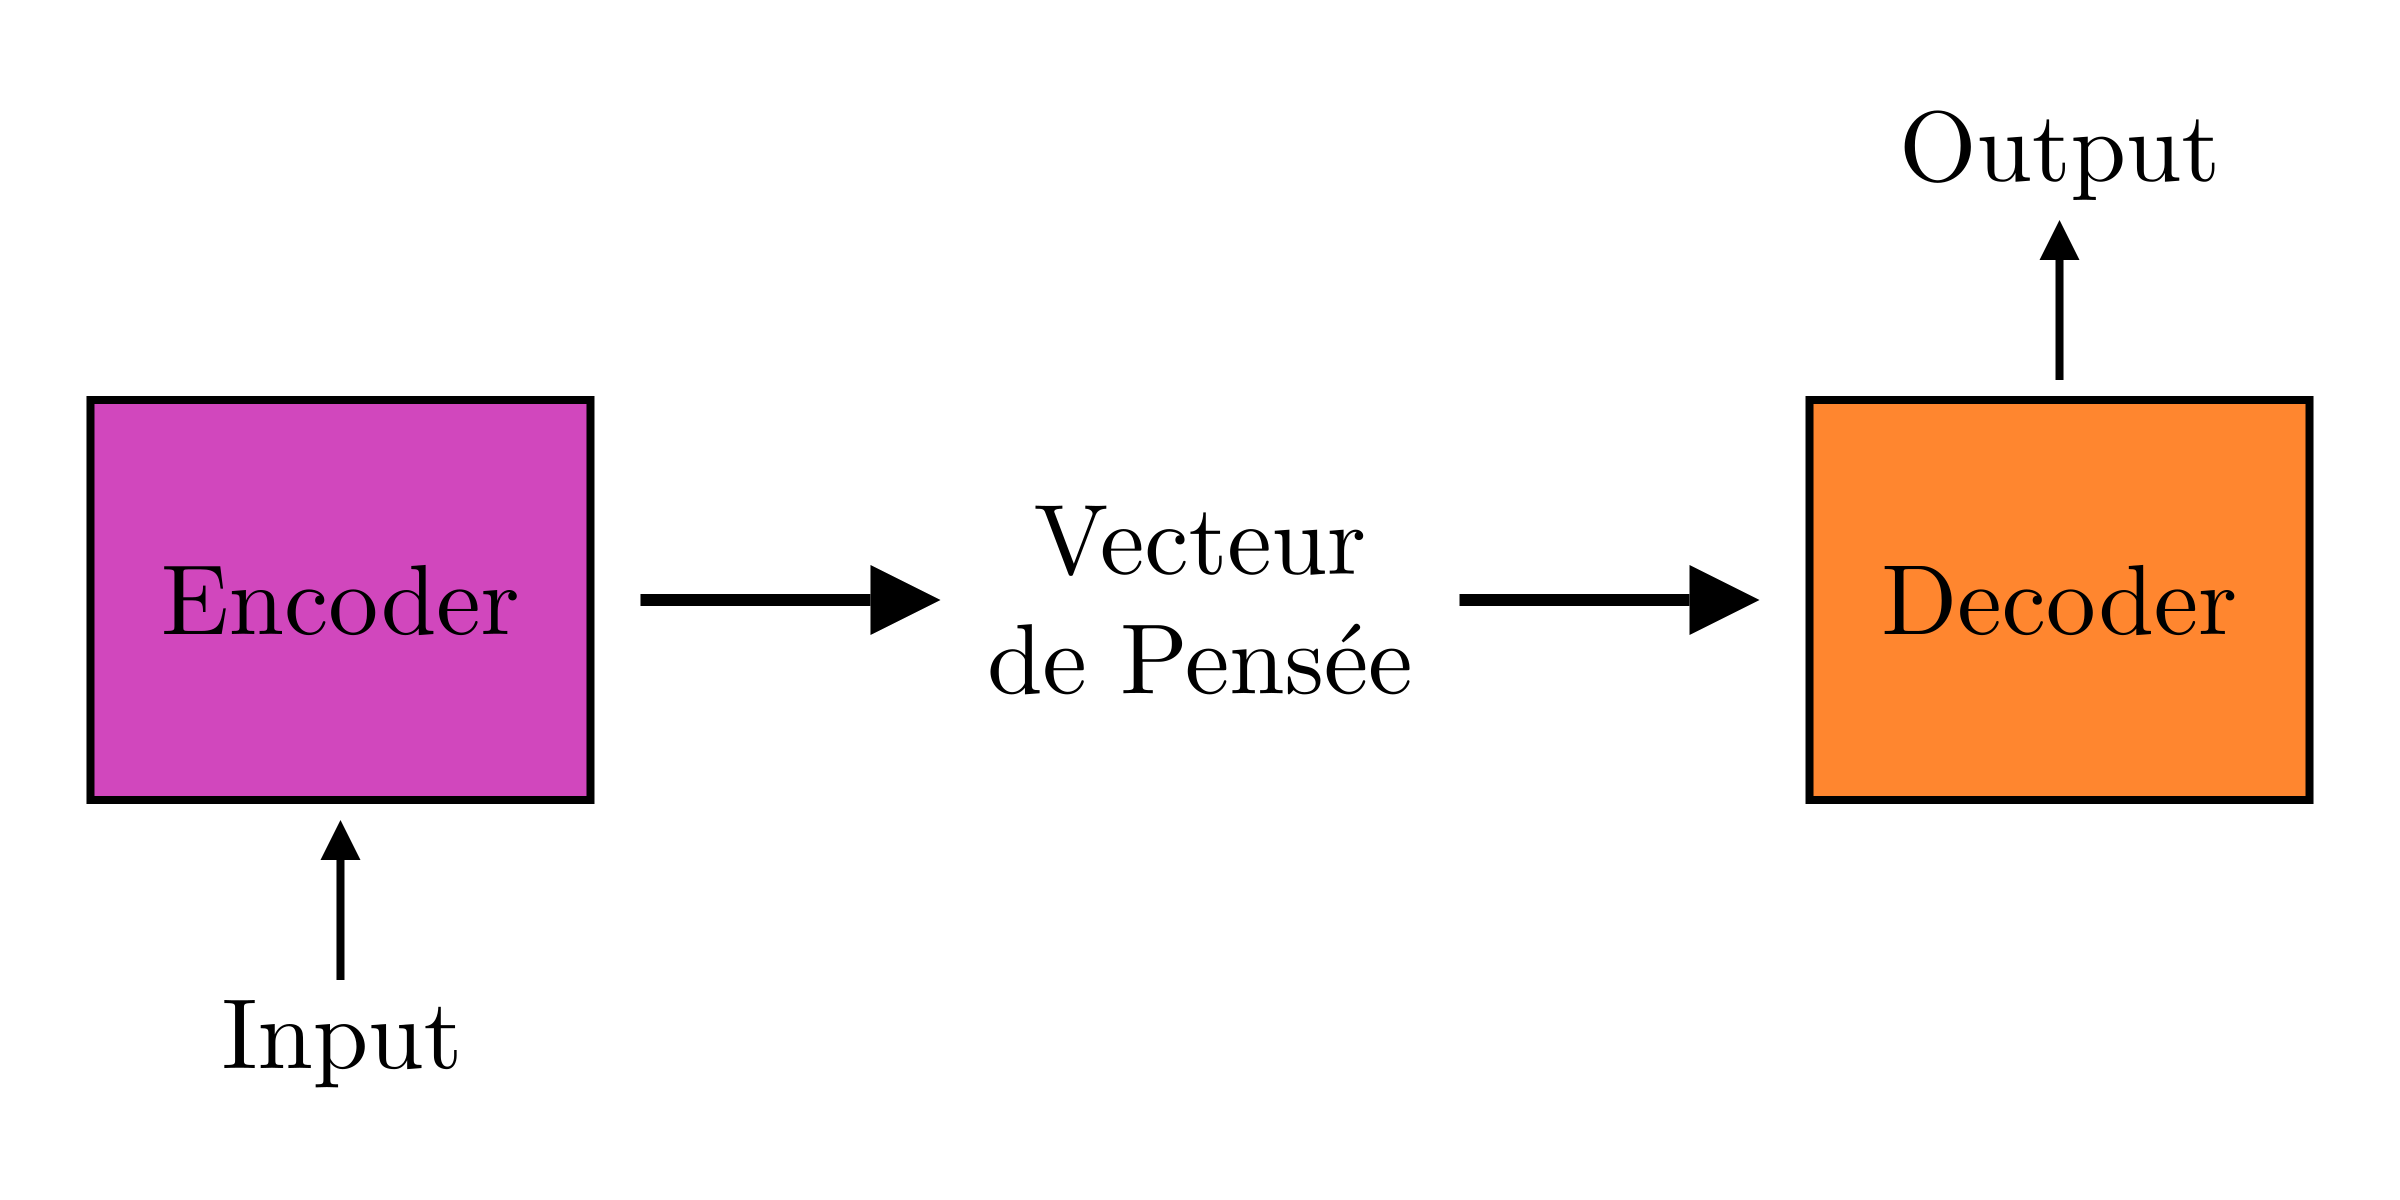
\includegraphics[width=10cm]{assets/images/encoder-decoder.png}
    \caption{Architecture encodeur--décodeur}
    \label{fig.encoder-decoder}
\end{figure}
%%
L'équation~\ref{eq.enc-dec} le montre sur le même exemple.
%%
\begin{equation}
    \label{eq.enc-dec}
    \begin{array}{l}
        c = \mathrm{econder}(x)\\
        y = \mathrm{decoder}(c)
    \end{array}
\end{equation}
%%

L'équation~\ref{eq.enc-dec} ne dépend ni du fonctionnement interne de l'encodeur ni de celui du décodeur.
Les deux modules peuvent avoir deux architectures quelconques, qui peuvent ou non être les mêmes~\cite{deep-nmt-survey}.
Dans le reste de ce chapitre, nous examinons les architectures communes en apprentissage \gls{s2s}.


% tenir compte de toute l'entrée à la pro
% produire chaque élément de la sortie en partant de l'entrée toute entière. 